\documentclass[11pt,a4paper]{article}
\usepackage[T1]{fontenc}\usepackage{lmodern}
\usepackage[margin=22mm,headheight=14pt]{geometry}
\usepackage{amsmath,amssymb,bm,booktabs,tabularx,array,graphicx,float,fancyhdr,microtype,xcolor}
\usepackage[colorlinks=true,linkcolor=blue!45!black,urlcolor=blue!45!black,citecolor=blue!45!black]{hyperref}
\setlength{\emergencystretch}{1em}\setlength{\parindent}{0pt}\setlength{\parskip}{5pt}\renewcommand{\arraystretch}{1.15}
\pagestyle{fancy}\fancyhf{}\fancyhead[L]{\small QFT Project B | Step 9}\fancyhead[R]{\small Group B}\fancyfoot[C]{\thepage}
\newcommand{\dd}{\mathrm{d}}
\begin{document}\hypersetup{pageanchor=false}
\begin{titlepage}\centering\vspace*{3mm}

\includegraphics[width=36mm]{assets/bits_logo.png}\par\vspace{13mm}
{\Large\bfseries BITS PILANI K.K. BIRLA GOA CAMPUS\par}\vspace{3mm}
{\large\bfseries Department of Physics\par}\vspace{18mm}
{\LARGE\bfseries What Quantum Trace Can\\[2mm] a Heavy Particle Leave?\par}\vspace{6mm}
{\large Curvature--Spectator Entanglement\\and the Cosmological Collider\par}\vspace{10mm}
{\large\bfseries Step 9: Mass Recovery and Fit Stability\par}\vspace{17mm}
{\Large\bfseries Group-B\par}\vspace{5mm}
\begin{tabular}{ll}Priyansh Rawat & 2023B5A70968G\\Mayank Sinha & 2023B5A70942G\\Samarth Bhatnagar & 2023B5A70853G\end{tabular}
\vfill{\large Under Professor: Rudranil Basu\par}\vspace{7mm}{29 October 2026\par}
\end{titlepage}\setcounter{page}{1}\hypersetup{pageanchor=true}
\section{Frequency profiling and mock-data calibration}
We fit
\begin{equation}F(r)=b_0+b_2r^2+r^{3/2}[A\cos(\mu\ln r)+B\sin(\mu\ln r)].\end{equation}
For each trial $\mu$, the remaining coefficients are linear. We scan $0.1\le\mu\le4$ in increments $0.01$, refine every local minimum and retain competing solutions. Known Gaussian mock errors define a profile likelihood; the nominal 95\% set is $\Delta\chi^2\le3.841459$, including disconnected intervals.
The mocks use 50 log-spaced points on $10^{-3}\le r\le0.2$, $M=2$, $g=0.1$, $A=0.1$, $B=0.05$, $b_0=0$, $b_2=0.2$. Their known frequency is $\sqrt{1.76}$. Independent noise has standard deviation 1\% or 5\% of the oscillatory RMS. Seed 20261029 gives 100 realisations at each noise level.
\begin{center}\small\begin{tabular}{llll}\toprule Noise & Frequency bias & Frequency RMSE & 95\% coverage\\\midrule
1\% & $0.002425$ & $0.04687$ & 93\%\\
5\% & $0.02179$ & $0.205$ & 94\%\\\bottomrule\end{tabular}\end{center}\begin{figure}[H]\centering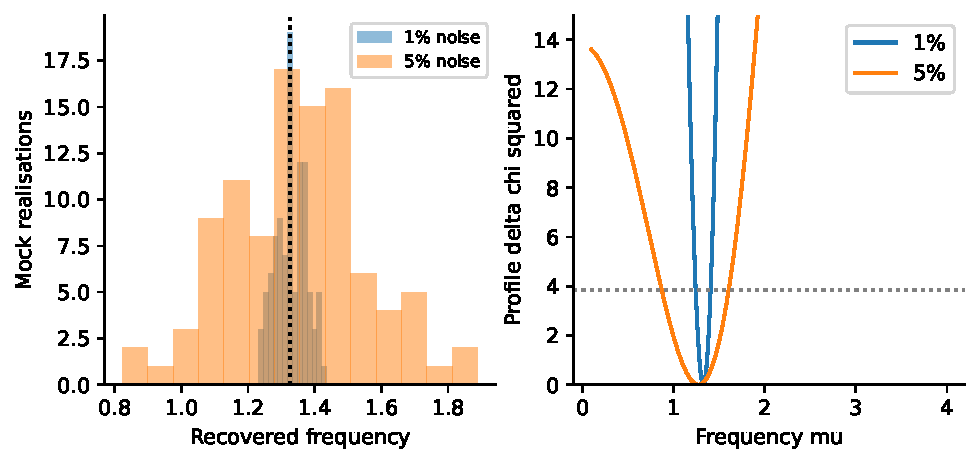
\includegraphics[width=.91\linewidth]{figures/mock_mass_recovery.pdf}\caption{Mock recovered frequencies and example profile curves. Coverage measures the mock likelihood procedure, rather than calibrating deterministic numerical errors in the physical calculation.}\end{figure}For a no-clock state, frequency is not identified, so a naive fixed-frequency significance test would miss the frequency search. We calibrate the improvement over the two-term background on 100 null realisations and test it on another 100 independent nulls per noise level. The held-out false-alarm rates are 2\% and 4\%. With 100 trials, differences of a few percentage points are not decisive.

\newpage
\section{Physical clock fit and finite-window limitations}
After the Step 8 pilot passes, we evaluate 50 physical triangles on $10^{-3}\le r\le0.2$. Regulator extrapolation is repeated at every point. The numerical weights combine the local regulator change with the other pilot error-budget contributions, interpolated in $\ln r$. They are deterministic accuracy diagnostics and do not define an observational statistical confidence interval.
\begin{figure}[H]\centering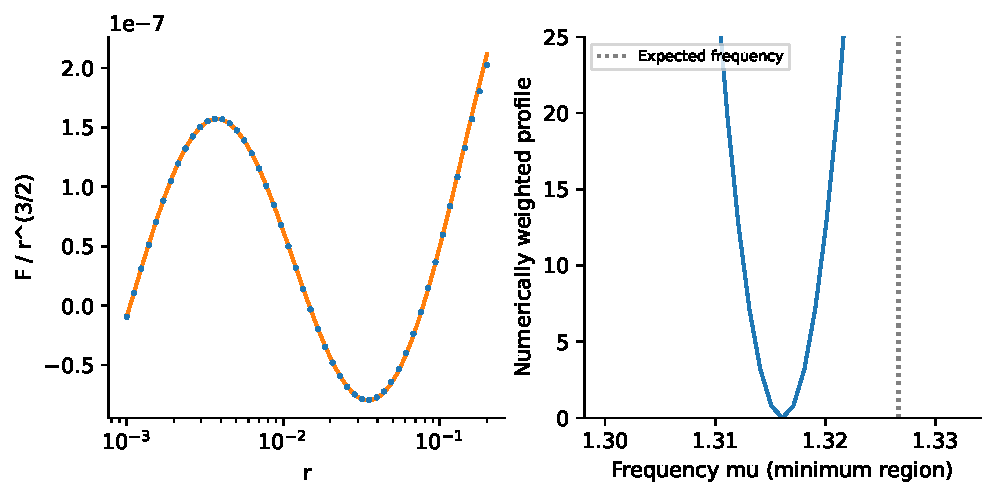
\includegraphics[width=.91\linewidth]{figures/physical_clock_fit.pdf}\caption{The physical bispectrum divided by $r^{3/2}$ and its numerical frequency profile. A narrow profile under one background choice does not include fit-model or window error.}\end{figure}\begin{sloppypar}The full-range leading fit has $\mu=1.316103$ and an oscillatory coefficient magnitude $\sqrt{A^2+B^2}=1.389\times10^{-7}$. The maximum numerical error divided by the fitted clock envelope is $0.008524$, below the 0.1 gate. However, only about $1.11$ cycles are visible, making the background model consequential.\end{sloppypar}
The late-time mass relation is
\begin{equation}m/H=\sqrt{\mu^2+9/4-g^2}.\end{equation}
Omitting $g^2$ is a weak-mixing approximation. If $g$ is unknown, the clock measures a mass--mixing combination.

\newpage
\section{Window and background stability}
We vary the upper endpoint $r_{\max}=0.05,0.1,0.2$, the lower endpoint $r_{\min}=0.001,0.003$, and add an $r^4$ analytic term as a background control. The resulting best fits are
\begin{center}\small\begin{tabular}{lllll}\toprule $r_{\min}$ & $r_{\max}$ & Extra $r^4$ & $\mu$ & $m/H$\\\midrule
$0.001$ & $0.05$ & no & $1.32317$ & $1.99769$\\
$0.001$ & $0.05$ & yes & $1.32544$ & $1.9992$\\
$0.003$ & $0.05$ & no & $1.31765$ & $1.99404$\\
$0.003$ & $0.05$ & yes & $1.32421$ & $1.99838$\\
$0.001$ & $0.1$ & no & $1.32041$ & $1.99587$\\
$0.001$ & $0.1$ & yes & $1.32445$ & $1.99854$\\
$0.003$ & $0.1$ & no & $1.31637$ & $1.9932$\\
$0.003$ & $0.1$ & yes & $1.32142$ & $1.99654$\\
$0.001$ & $0.2$ & no & $1.3161$ & $1.99302$\\
$0.001$ & $0.2$ & yes & $1.32196$ & $1.99689$\\
$0.003$ & $0.2$ & no & $1.35637$ & $2.01983$\\
$0.003$ & $0.2$ & yes & $1.31787$ & $1.99419$\\\bottomrule\end{tabular}\end{center}
The best-fit frequency envelope is $1.3161$--$1.35637$, corresponding to a mass envelope $1.99302$--$2.01983$. This is a sensitivity range across the specified analyses, not a confidence interval with demonstrated coverage.
The expected $\mu=1.326649916$ lies in this range. Restricting to the more squeezed $r\le0.05$ interval with the added analytic term produces a closer central estimate, while reducing the interval also weakens identifiability. We therefore report a resolved heavy-clock shape with model-dependent mass precision, rather than selecting the narrowest profile as the final error. The calibrated mock recovery and the physical numerical fit answer different questions.\begin{thebibliography}{9}\small
\bibitem{collider} N. Arkani-Hamed and J. Maldacena, \emph{Cosmological Collider Physics}, \href{https://arxiv.org/abs/1503.08043}{arXiv:1503.08043}.\end{thebibliography}
\textbf{Code and supporting data:} \href{https://github.com/rawatpriyansh17/QFT-PROJECT-GROUP-B/tree/main/step9}{step9 on GitHub}.\newpage\section*{Contributions (equal)}\begin{center}\begin{tabularx}{\linewidth}{p{33mm}X}\toprule Member & Contribution\\\midrule Priyansh Rawat & Frequency model and mass-conversion interpretation.\\[3mm]Samarth Bhatnagar & Mock/no-clock calibration and fit-window review.\\[3mm]Mayank Sinha & Profile fitting, physical shape scan and figures.\\\bottomrule\end{tabularx}\end{center}\end{document}